\section{Introduction}

A standard problem in psycholinguistics\pb{not really limited to psychology...processes unfolding in time are pretty ubiquitous throughout science}, and the cognitive sciences in general, is that of statistically analyzing a process unfolding in time. Particularly in the case of comparing a process between experimental groups in time, while there are many appropriate techniques for demonstrating that differences \textit{exist}, such as comparing the area under the curve (AUC) of the two processes or testing for differences in the underlying parameters (if the process is being modeled in a parametric manner). However, these offer little insight with respect to identifying \textit{when} these processes are significantly different, which is often the more relevant scientific question. Testing for time differences is complicated by the fact that there are effectively an infinite number of time points that could be compared, with the test results at nearby time points highly correlated. Both of these factors complicate efforts to correct for multiple comparisons.

Various approaches have been proposed, such as using cluster based permutation testing \cite{Maris2007}. Here, test-statistics are computed at each time, with adjacent significant tests being combined into clusters. This controls for the family wise error rate (FWER) by reducing adjacent test statistics into a single cluster, thereby reducing the number of tests. More recently, \cite{oleson2017detecting} used bootstrapped fits of subject-level curves and estimated the correlation structure of the test statistics in order to modify the Bonferroni correction of the significance level to control FWER. This approach, which they named bootstrapped differences of time series, was introduced in the R package \xt{bdots} \citep{seedorff2018bdots}.

A closer look at the specific conditions under which the original iteration of \xt{bdots} was presented raises concerns, however, involving quite restrictive assumptions that are unlikely to be met in many, if not most, situations. This includes data typically collected in the Visual World Paradigm (VWP), context in which the underlying methodology was first proposed. Specifically, it assumed a homogeneous mean structure within each of the groups being compared, with no between-subject variability to be accounted for. Empirical data collected in a variety of (VWP) contexts can be used to show that such an assumption is unlikely to be true, with the resulting type I error rate being unacceptably high.

Here, we present two alternatives that accommodate flexibility in the assumptions made by the original bdots. First, we propose a modified bootstrapping procedure that adequately accounts for observed between subject variability while retaining the FWER adjustment method presented for autocorrelated errors. In addition, we offer a permutation test between the groups, borrowing from the insight of the original bdots in that it also captures within-subject variability as demonstrated in the standard errors in the model fits. We begin by describing the two proposed alternatives to the original bdots bootstrap. We then outline the details of the simulations in demonstrating the type I error rate across a number of experimental conditions, and finally we conclude with a demonstration of power in the competing methods.

\section{Methods}

\pb{Define data notation here. we observe $y_{it}$ for subjects $i=1, \ldots, n$ over times $t=1, \ldots, T$. typically fall into separate groups and we want to compare those groups}

\subsection{Homogeneous bootstrap}

\pb{revise this in light of above} Most generally the original bdots algorithm, which we will call the \textit{homogeneous bootstrap}, proposed that we have empirically observed data in time resulting from a parametric function $f$ with an associated error: 

\begin{equation}\label{eq:mean_structure}
y_{it} = f(t|\theta) + \epsilon_{it}
\end{equation}
where 
\begin{equation}
\epsilon_{it} = \phi \epsilon_{i, t-1} + w_{it}, \quad w_{it} \sim N(0, \sigma).
\end{equation}
Under this paradigm, the errors could be iid normal (with $\phi = 0$) or have an AR(1) structure, with $0 < \phi < 1$. It further assumes homogeneity of the mean structure, meaning that if subjects $i$ and $j$ are from the same group, we have \pb{this kind of thing does not work at all -- you define $\theta$ above. it has no subscripts. You can't just refer to $\theta_{it}$ all of a sudden -- it's never been defined. Also, $\theta$ doesn't depend on $t$ at all, in any scenario. $\theta_{it} = \theta_{jt}$}. In other words, there is no variability in the mean structure between subjects, only between groups. \cn{This is also evidenced in the original bdots algorithm: }

%\begin{singlespace}
\pb{why are you manually numbering?}
\begin{enumerate}
\vspace{-3mm}
\item For each subject, fit a nonlinear regression model to obtain $\hat{\theta}_i$. \cite{oleson2017detecting} recommended specifying an AR(1) autocorrelation structure for model errors. Assuming large sample normality, the sampling distribution of each estimator can be approximated by a normal distribution with mean corresponding to the point estimate and standard deviation corresponding to the standard error.

\item Using the approximate sampling distributions in (1.), randomly draw one bootstrap estimate for each of the model parameters on every subject \pb{MATH: $\hat{\theta}_i^{(b)} \sim ()$ or so}.

\item Once a bootstrap estimate has been collected for each parameter and for every subject, for each parameter, find the mean of the bootstrap estimates across individuals  \pb{MATH}.

\item Use the mean estimates to determine the predicted population level curve, which provides the average population response at each time point.   \pb{MATH}

\item Perform steps (2)-(4) 1000 times to obtain estimates of the population curves. Use these to create estimates of the mean response and standard deviation at each of the time points.  \pb{MATH}.
\end{enumerate}
%\end{singlespace}

Population means and standard deviations at each time point for each of the groups were used to construct a series of (correlated) test statistics, where the family wise error rate was controlled by using the modified Bonferonni correction introduced in \cite{oleson2017detecting} to test for significance. \pb{This modified correction seems kind of important (among other things, hetboot uses it too), I think you should say more about it}

\subsection{Heterogeneous Bootstrap}

Typically, subjects within a group demonstrate considerable variability in their mean parameter estimates. In this case, we should avoid the presumption that $\theta_i = \theta_j$, since accounting for between-subject variability within a group will be critical for obtaining a reasonable distribution of the population curves.

Instead of \eqref{}

\label{eq:mean_structure}
\cn{A more likely case involving subjects in the VWP (or subjects within any group exhibiting between and within subject variability) is as such: }

The distribution of parameters for subjects $i = 1, \dots, n_g$ in group $g = 1, \dots, G$ follows the distribution

\begin{equation}\label{eq:theta_i_dist}
\theta_i \sim N(\mu_{g}, V_{g}).
\end{equation}

The uncertainty present in our estimation of $\theta_i$ can be accounted for by treating the standard errors derived when fitting the observed subject data to Equation~\ref{eq:mean_structure} as estimates of their standard deviations. This gives us a distribution for the subject's estimated parameter, 

\begin{equation}
\hat{\theta}_i \sim N(\theta_i, s_i^2).
\end{equation}

When obtaining reasonable estimates of the population curve, it is necessary to estimate both the observed within-subject variability found in each of the $\{s_i^2\}$ terms, \textit{as well as} the between-subject variability present in $V_{g}$. For example, let $\theta^*_{ib}$ represent a bootstrapped sample for subject $i$ in bootstrap $b = 1, \dots, B$, where

\begin{equation}\label{eq:sub_boot_dist}
\theta^*_{ib} \sim N(\hat{\theta}_i, s_i^2).
\end{equation}
If we were to sample \textit{without replacement}, we would obtain a homogeneous mean value from the $b$th bootstrap for group $g$, $\theta^{(hom)}_{bg}$, where

\begin{equation}\label{eq:wo_rep_boot}
\theta^{(hom)}_{bg} = \frac{1}{n_g} \sum \theta^{*}_{ib}, \quad \theta^{(hom)}_{bg} \sim N \left( \mu_{g}, \frac{1}{n_g^2} \sum s_i^2 \right).
\end{equation}

Such an estimate captures the totality of the within-subject variability with each draw but fails to account for the variability in the group overall. For this reason, we sample the subjects \textit{with} replacement, creating the heterogeneous bootstrap mean $\theta_{bg}^{(het)}$, where again each $\theta_{ib}^*$ follows the distribution in Equation~\ref{eq:sub_boot_dist}, but the heterogeneous bootstrapped group mean now follows

\begin{equation}\label{eq:w_rep_boot}
\theta_{bg}^{(het)} \sim N \left( \mu_{g}, \frac{1}{n_g} V_{g} + \frac{1}{n_g^2} \sum s_i^2 \right).
\end{equation}

The estimated mean value remains unchanged, but the variability is now fully accounted for. We therefore present a modified version of the bootstrap which we call the \textit{heterogeneous bootstrap}, making the following changes to the original: \cn{make equations for this}

%\begin{singlespace}
\begin{enumerate}
%.\vspace{-2mm}
\item[1.] In step (1.), the specification of AR(1) structure is \textit{optional} and can be modified with arguments to functions in \xt{bdots}. Our simulations show that while failing to include it slightly inflates the type I error in the v2 bootstrap when the data truly is autocorrelated, specifying an AR(1) structure can lead to overly conservative estimates when it is not.
\item[2.] In step (2.), we sample subjects \textit{with replacement} and then for each drawn subject, randomly draw one bootstrap estimate for each of their model parameters based on the mean and standard errors derived from the \xt{gnls} estimate.
\end{enumerate}
%\end{singlespace}

Just as with the homogeneous bootstrap, these bootstrap estimates are used to create test statistics $T_t$ at each time point, written

\begin{equation}
T_t^{(b)} = \frac{(\overline{p}_{1t} - \overline{p}_{2t})}{\sqrt{s_{1t}^2 + s_{2t}^2}},
\end{equation}

where $\overline{p}_{gt}$ and $s_{gt}^2$ are mean and standard deviation estimates at each time point for groups $1$ and $2$, respectively. Finally, just as in Oleson 2017, one can use the autocorrelation of the $T_t^{(b)}$ statistics to create a modified $\alpha$ for controlling the FWER.



\cn{A paired bootstrapping can be implemented by performing this same algorithm but ensuring that at each iteration of the bootstrap the same subjects are sampled with replacement in each group. This happened by default in the original implementation as each subject was retained in each iteration of the bootstrap.}


\subsection{Permutation Testing}

In addition to the heterogeneous bootstrap, we also introduce a permutation method for hypothesis testing. The permutation method proposed is analogous to a traditional permutation method, but with an added step mirroring that of the previous in capturing the within-subject variability. For a specified FWER of $\alpha$, the proposed permutation algorithm is as follows:

\cn{need to add math here}

%\begin{singlespace}
\begin{enumerate}
\vspace{-2mm}
\item For each subject, fit the nonlinear function with \textit{optional} AR(1) autocorrelation structure for model errors. Assuming large sample normality, the sampling distribution of each estimator can be approximated by a normal distribution with mean corresponding to the point estimate and standard deviation corresponding to the standard error
\item Using the mean parameter estimates derived in (1.), find each subject's corresponding fixation curve. Within each group, use these to derive the mean and standard deviations of the population level curves at each time point, denoted $\overline{p}_{jt}$ and $s_{jt}^2$ for $j = 1,2$. Use these values to compute a test statistic $T_t$ at each time point,

\begin{equation}
T_t^{(p)} = \frac{|\overline{p}_{1t} - \overline{p}_{2t}|}{\sqrt{s_{1t}^2 + s_{2t}^2}}.
\end{equation}
This will be our observed test statistic.
\item Repeat (2) $P$  additional times, each time shuffling the group membership between subjects. This time, when constructing each subject's corresponding fixation curve, draw a new set of parameter estimates using the distribution found in (1). Recalculate the test statistics $T_t^{(p)}$, retaining the maximum value from each permutation. This collection of $P$ statistics will serve as our null distribution which we denote $\widetilde{T}$. Let $\widetilde{T}_{\alpha}$ be the $1$ - $\alpha$ quantile of $\widetilde{T}$
\item Compare each of the observed $T_t^{(p)}$ with $\widetilde{T}_{\alpha}$. Areas where $T_t^{(p)} > \widetilde{T}_{\alpha}$ are designated significant. 
\end{enumerate}
%\end{singlespace}

Paired permutation testing is implemented with a minor adjustment to step (3). Instead of permuting all of the labels between groups, randomly assign each subject to either retain their current group membership or to change groups. This ensures that each permuted group contains one observation from each subject.



\section{Type I Error Simulations}

We now go about comparing the type I error rate of the three methods just described. In doing so, we will consider several conditions under which the observed subject data may have been generated or fit. This includes two conditions for the mean structure, two conditions for the error structure, paired and unpaired data, and data fit with and without an AR(1) assumption. Considering each permutation of this arrangement results in sixteen different settings. Each simulation will then be examined for type I error using each of the three methods described.



\subsection{Data Generation}

Data was generated according to Equation~\ref{eq:mean_structure}, with the parametric function $f(t|\theta)$ belonging to the family of four-parameter logistic curves defined:

\begin{equation}\label{eq:logistic}
f(t | \theta) = \frac{p-b}{1 + \exp \left(\frac{4s}{\text{p}-b} (x - t) \right)} + b
\end{equation}
where $\theta = (p, b, s, x)$, the peak, baseline, slope, and crossover parameters, respectively.


\begin{figure}
    \centering
    \subfigure[]{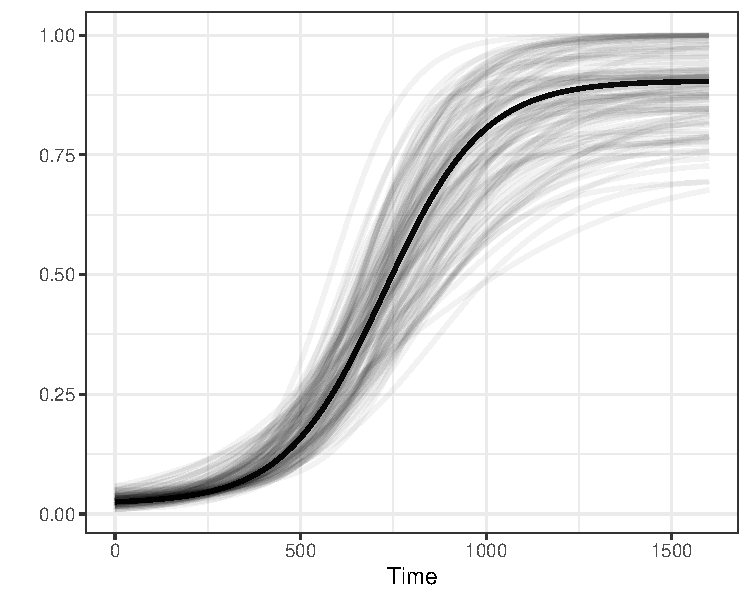
\includegraphics[width=0.45\textwidth]{logistic_distribution.pdf}} 
    \subfigure[]{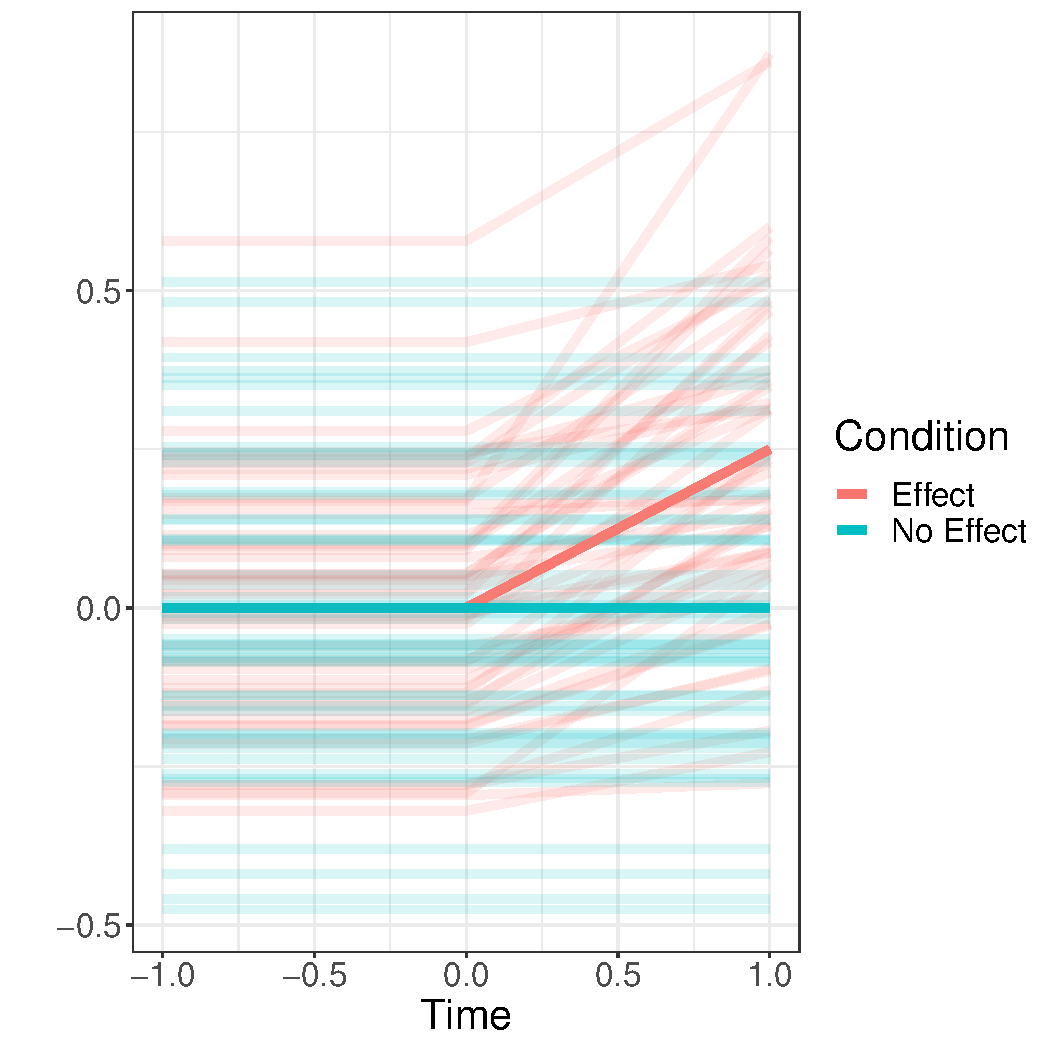
\includegraphics[width=0.45\textwidth]{piecewise_distribution.pdf}}
    \caption{Distributions of various group with the mean curve in bold (a.) 50 samples from the generating distribution of the four-parameter logistic in Equation~\ref{eq:logistic} used for testing FWER. (b.) 50 samples from the generating distributions of each group in Equation~\ref{eq:piecewise_form}. The legend makes size weird, might just explain what they are here. Also need to see if I can change size of the mean lines}
\label{fig:distribution}
\end{figure}



We further assume that each group drew subject-specific parameters from a normal distribution, with subject $i = 1, \dots, N$ in group $g = 1, \dots, G$ following the distribution in Equation~\ref{eq:theta_i_dist}.

\cn{Could also expression this $\theta_i^{(g)}$? Though that may be cumbersome}

\paragraph{Mean Structure} In all of the simulations presented, the distribution used in Equation~\ref{eq:tie_dist} was empirically determined from data on normal hearing subjects in the VWP (Farris-Trimble et  al., 2014 \cite{FarrisTrimble2014}). Parameters used were those fit to fixations on the Target, following the functional form of Equation~\ref{eq:logistic}. Under the assumption of between-subject homogeneity, we set $\theta_i = \theta_j$ for all subjects $i,j$, assuring that each of the subjects' observations is derived from the same mean structure, differing only in their observed error. We will call this the homogeneous means assumption.


\paragraph{Error Structure} The error structure is of the form

\begin{equation}
e_{it} = \phi e_{i, t-1} + w_{it}, \quad w_{it} \sim N(0, \sigma)
\end{equation}
where the $w_{it}$ are iid with $\sigma = 0.025$. $\phi$ corresponds to an autocorrelation parameter and is set to $\phi = 0.8$ when the generated data is to be autocorrelated and set to $\phi = 0$ when we assume the errors are all independent and identically distributed. 

\paragraph{Paired Data} Finally we considered paired data, though this is only a sensible condition under the assumption of heterogeneous means. In order to construct paired data, we simply used the same parameter estimates for each subject between groups, with the observed data between subjects differing only in the observed error.


Each set of conditions generates two groups, with $n = 25$ subjects in each group, with timepoints $t = 0, 4, 8, \dots, 1600$ in each trial and with $100$ simulated trials for each subject. Columns in the tables indicate homogeneity of means assumption, whether or not an AR(1) error structure was used in constructing the data, and if autocorrelation was specified in the fitting function. The last conditions helps assess the impact of correctly identifying the type of error when conducting an analysis in \xt{bdots}. Each simulation was conducted 100 times to determine the rate of type I error (time intensive and will launch 1000 for final dissertation). 


\subsection{Results}

We consider the efficacy the methods under each of the simulation settings with an analysis of the family wise error rate (FWER) and the median per-comparison error rate. The first of these details the proportion of simulations under each condition that marked \textit{at least} one time point as being significantly different between the two groups. This is critical is understanding each method's ability to correct adjust for the multiple testing problem associated with testing each of the observed time points. These are presented in Table~\ref{tab:fwer_unpaired} and Table~\ref{tab:fwer_paired} for unpaired and paired data, respectively.

Complimenting the FWER estimate is an estimate of the median per-comparison rate. For each time point across each of the simulations, we computed the proportion of times in which that time was determined significant. The median of these values across all time points is what is considered. This metric gives a sense of magnitude to the binary FWER; for example, a situation in which there was a high FWER and low median per-comparison rate would indicate that the type I error within a particular time series would be sporadic and impact limited regions. Large median per-comparison rates indicate that large swaths of a time series frequently sustain type I errors. The median per-comparison rates for unpaired and paired simulations are presented in Table~\ref{tab:mpc_unpaired} and Table~\ref{tab:mpc_paired}.


\subsubsection{FWER}



There are a few things of immediate note when considering the results of Table~\ref{tab:fwer_unpaired}. First, we see from the first two settings of the unpaired simulations that the type I error rates for the homogenous bootstrap are consistent with those presented in \cite{oleson2017detecting}, confirming the importance of specifying the existence of autocorrelation in the \xt{bdots} fitting function when autocorrelated error is present. By contrast, this is far less of a concern when using the heterogeneous bootstrap or permutation testing, both of which maintain a FWER near the nominal alpha, regardless of whether or not the error structure was correctly identified. This continues to be true under the homogenous mean assumption when the true error structure is not autocorrelated. Interestingly, the performance of the homogeneous bootstrap falters here despite theoretical consistency with the simulation settings. \cn{I am rerunning this condition again now to make sure there wasn't an error.}

The most striking results of this, however, appear when the data generation assumes a heterogeneous mean structure. While both the heterogeneous bootstrap and the permutation test maintain a FWER near the nominal alpha, the homogeneous bootstrap fails entirely, with a FWER $> 0.9$ in all cases.

\begin{table}[H]
\centering
\begin{tabular}{cccccc}
  \hline
  \multicolumn{1}{p{2cm}}{\centering Heterogeneity \\ Assumption} & \multicolumn{1}{p{2cm}}{\centering Autocorrelated \\ Error} & \multicolumn{1}{p{2cm}}{\centering AR(1)  \\ Specified} &  \multicolumn{1}{p{2cm}}{\centering Homogeneous \\ Bootstrap} &\multicolumn{1}{p{2cm}}{\centering Heterogeneous \\ Bootstrap} & \multicolumn{1}{p{2cm}}{\centering Permutation } \\ 
  \hline
No & Yes & Yes & 0.06 & 0.01 & 0.08 \\ 
  No & Yes & No & 0.87 & 0.08 & 0.00 \\ 
  No & No & Yes & 0.08 & 0.00 & 0.06 \\ 
  No & No & No & 0.15 & 0.02 & 0.01 \\ 
  Yes & Yes & Yes & 0.92 & 0.03 & 0.05 \\ 
  Yes & Yes & No & 0.96 & 0.02 & 0.08 \\ 
  Yes & No & Yes & 0.99 & 0.05 & 0.03 \\ 
  Yes & No & No & 1.00 & 0.05 & 0.06 \\  
   \hline
\end{tabular}
\caption{FWER for empirical parameters (unpaired)}
\label{tab:fwer_unpaired}
\end{table}

Paired data is given in Table~\ref{tab:fwer_paired}. Matching the conclusions drawn from Table~\ref{tab:fwer_unpaired}, we only note here that both the permutation test and heterogeneous bootstraps maintain a valid FWER under the assumption of paired data.

\begin{table}[H]
\centering
\begin{tabular}{cccccc}
  \hline
  \multicolumn{1}{p{2cm}}{\centering Heterogeneity \\ Assumption} & \multicolumn{1}{p{2cm}}{\centering Autocorrelated \\ Error} & \multicolumn{1}{p{2cm}}{\centering AR(1) \\ Specified} &  \multicolumn{1}{p{2cm}}{\centering Homogeneous \\ Bootstrap} &\multicolumn{1}{p{2cm}}{\centering Heterogeneous \\ Bootstrap} & \multicolumn{1}{p{2cm}}{\centering Permutation } \\  
  \hline
  Yes & Yes & Yes & 0.49 & 0.02 & 0.01 \\ 
  Yes & Yes & No & 0.94 & 0.03 & 0.02 \\ 
  Yes & No & Yes & 0.72 & 0.02 & 0.00 \\ 
  Yes & No & No & 0.74 & 0.04 & 0.00 \\ 
   \hline
\end{tabular}
\caption{FWER for empirical parameters (paired)}
\label{tab:fwer_paired}
\end{table}

\subsubsection{Median per comparison error rate}

We next consider the median comparison rate, which offers some insight into the FWER. In particular, consider the situation in which in Table~\ref{tab:mpc_unpaired}, in the fourth row we see a median per-comparison error rate of 0.00 for the homogeneous bootstrap, despite Table~\ref{tab:fwer_unpaired} indicating a FWER of 0.15. This is a consequence of the majority of the type I errors occuring in a relatively limited region. In contrast, the median per-comparison error rate of the homogeneous bootstrap under the assumption of heterogeneity suggests that the type I errors are widespread and not limited to any particular area. 

It is also worth commenting on the permutation test median per-comparison error rate in Table~\ref{tab:mpc_unpaired}; combined with a FWER near the nominal 0.05, these values suggest that errors are likely distributed across the entire range rather than limited to a small area (which would result in a MPCR of 0). 

\cn{I confirmed this by looking both at this histograms and inspecting the data manually}

\begin{table}[H]
\centering
\begin{tabular}{cccrrr}
  \hline
  \multicolumn{1}{p{2cm}}{\centering Heterogeneity \\ Assumption} & \multicolumn{1}{p{2cm}}{\centering Autocorrelated \\ Error} & \multicolumn{1}{p{2cm}}{\centering  AR(1) \\ Specified} &  \multicolumn{1}{p{2cm}}{\centering Homogeneous \\ Bootstrap} &\multicolumn{1}{p{2cm}}{\centering Heterogeneous \\ Bootstrap} & \multicolumn{1}{p{2cm}}{\centering Permutation } \\ 
  \hline
No & Yes & Yes & 0.01 & 0.00 & 0.04  \\ 
  No & Yes & No & 0.31 & 0.00 & 0.04 \\ 
  No & No & Yes & 0.00 & 0.00 & 0.02\\ 
  No & No & No & 0.00 & 0.00 & 0.03 \\ 
  Yes & Yes & Yes & 0.51 & 0.01 & 0.01 \\ 
  Yes & Yes & No & 0.76 & 0.01 & 0.00 \\ 
  Yes & No & Yes & 0.86 & 0.01 & 0.00 \\ 
  Yes & No & No & 0.81 & 0.01 & 0.00 \\ 
   \hline
\end{tabular}
\caption{median per comparison error rate (unpaired)}
\label{tab:mpc_unpaired}
\end{table}



\begin{table}[H]
\centering
\begin{tabular}{cccrrr}
  \hline
  \multicolumn{1}{p{2cm}}{\centering Heterogeneity \\ Assumption} & \multicolumn{1}{p{2cm}}{\centering Autocorrelated \\ Error} & \multicolumn{1}{p{2cm}}{\centering AR(1) \\ Specified} &  \multicolumn{1}{p{2cm}}{\centering Homogeneous \\ Bootstrap} &\multicolumn{1}{p{2cm}}{\centering Heterogeneous \\ Bootstrap} & \multicolumn{1}{p{2cm}}{\centering Permutation } \\ 
  \hline
  Yes & Yes & Yes & 0.13 & 0.00 & 0.00 \\ 
  Yes & Yes & No & 0.52 & 0.02 & 0.00 \\ 
  Yes & No & Yes & 0.38 & 0.01 & 0.00 \\ 
  Yes & No & No & 0.44 & 0.01 & 0.00 \\ 
   \hline
\end{tabular}
\caption{median per comparison error rate (paired)}
\label{tab:mpc_paired}
\end{table}


\subsection{Discussion}

Table~\ref{tab:fwer_unpaired} and Table~\ref{tab:fwer_paired} demonstrate that under a variety of settings, both the heterogeneous bootstrap and permutation offer a FWER near the nominal alpha, making their performance similar to that of the homogeneous bootstrap in the best of cases. This includes less restrictive assumptions in which they continue to perform well while the homogeneous bootstrap maintains an unacceptably high FWER. 

Transition sentence to power simulations

\section{Power Simulations}


To determine power, two experimental groups were simulated with mean structures of the following form:

\begin{equation}\label{eq:piecewise_form}
y = \begin{cases}
b \quad &x < 0 \\
mx + b \quad &x \geq 0
\end{cases}
\end{equation}

The first simulated group was ``No Effect", with intercept and slope parameters normally distributed and standard deviation $\sigma = 0.05$. The second group, the ``Effect" group, was similarly distributed, but with the slope parameter having mean value of $\mu = 0.25$. The error structure was identical to that in the FWER simulations, with both an AR(1) error structure and independent noise included. 100 simulations were conducted for each scenario. 

We limited consideration to three possible scenarios: first, we assumed the conditions presented in Oleson 2017, assuming homogeneity between subject parameters and an AR(1) error structure, with the model fitting performed assuming autocorrelated errors. For the remaining scenarios, we assumed heterogeneity in the distribution of subject parameters, simulated with and without an AR(1) error structure. In both of these last two scenarios, we elected to \textit{not} fit the model assuming autocorrelated errors. This was for two reasons: first, simulations exploring the type I error rate suggested that models fit with the autocorrelation assumption tended to be conservative. Second, and given the results of the first, this makes setting the assumption of autocorrelation to FALSE in \xt{bdots} seem like a sensible default, and as such, it would be of interest to see how the model performs in cases in which their is autocorrelated error that is not accounted for.

For each subject, parameters for their mean structure given in Equation~\ref{eq:piecewise_form} were drawn according to their group membership and fit using \xt{bdots} on the interval (-1,1). Time windows in which the groups differed were identified using each the homogenous bootstrap, heterogeneous bootstrap, and permutation testing. By including the interval (-1,0) in which the null hypothesis was true, we are able to mitigate the effects of over-zealous methods in determining power, and we present the results in the following way: any tests in which a difference was detected in (-1,0) was marked as having a type I error, and the proportion of simulations in which this occurred for each method is reported as the FWER in the column labeled $\alpha$. The next column, $\beta$, is the type II error rate, indicating the proportion of trials in which no differences were identified over the entire region. The last Greek-letter column is $1 - \beta - \alpha$, a modified power statistic indicating the proportion of tests in which a difference was correctly identified. The remaining columns relate to this modified power columns, giving a partial summary of the earliest onset of detection. As a true difference occurs on the interval $t > 0$, smaller values indicate greater power in detecting differences. Finally, a plot giving the power at each time point is given in Figure~\ref{fig:time_power_plot}. This plot represents the true power, though note that it does not take into account the rate at which these regions were identified in conjunction with a type I error rate.


\subsection{Results}

[tables up until this point had \textit{actually} been run with incorrect slope (0.025 instead of 0.25). Presented here now (3/5) are the correct tables. None of the results changed materially, though the type II error is much lower (given the corrected larger effect). Additionally, the current results only include 200 simulations. For completeness, I am running the full suite of simulations with both $m = 0.025$ and $m = 0.25$, though the only difference, again, will be in type II error and onset of detection]

The results of the power simulation are presented in Table~\ref{tab:power_methods}. We begin by considering the case in which we assumed a homogeneous mean structure with autocorrelated errors (the first three rows), matching the conditions in which the homogeneous bootstrap was first presented. Notably, we find that the permutation method demonstrates the greater power, with the median onset time just under that of the homogeneous bootstrap. This is at the expense of a larger FWER, though still below the nominal level. Alternatively, the heterogeneous bootstrap maintains a similar FWER as the homogeneous bootstrap at the cost of power.

The remaining settings tell a similar story with the exception of the homogeneous bootstrap which continues to demonstrate unacceptable FWER under the heterogeneous means assumption. We also seem some effect of not correctly specifying an AR(1) error structure when comparing the last two settings, as the failure to specify resulted in a slightly higher FWER and lower power, although not significantly (see Appendix for tables and figures of remaining situations). 


% latex table generated in R 4.2.2 by xtable 1.8-4 package
% Sat Feb 18 14:03:58 2023
\begin{table}[H]
\centering
\begin{tabular}{lcccccccc}
  \hline
Method & Heterogeneity & AR(1) & $\alpha$ & $\beta$ & 1 - $\alpha$ - $\beta$ & 1st Qu. & Median & 3rd Qu. \\ 
  \hline
Hom. Boot & No & Yes & 0.00 & 0.00 & 1.00 & 0.025 & 0.030 & 0.035 \\ 
  Het. Boot & No & Yes & 0.00 & 0.00 & 1.00 & 0.035 & 0.040 & 0.045 \\ 
  Perm & No & Yes & 0.03 & 0.00 & 0.97 & 0.020 & 0.025 & 0.030 \\
  \hline
  Hom. Boot & Yes & No & 0.95 & 0.00 & 0.05 & 0.005 & 0.008 & 0.010 \\ 
  Het. Boot & Yes & No & 0.00 & 0.01 & 0.98 & 0.260 & 0.330 & 0.480 \\ 
  Perm & Yes & No & 0.04 & 0.00 & 0.95 & 0.245 & 0.325 & 0.452 \\
  \hline
  Hom. Boot & Yes & Yes & 0.94 & 0.00 & 0.06 & 0.005 & 0.013 & 0.015 \\ 
  Het. Boot & Yes & Yes & 0.01 & 0.01 & 0.98 & 0.270 & 0.370 & 0.465 \\ 
  Perm & Yes & Yes & 0.04 & 0.00 & 0.96 & 0.245 & 0.365 & 0.440 \\ 
   \hline
\end{tabular}
\caption{Power for methods, updated (3/5). Note that with the slope being 0.25, nearly all methods detect difference within interval. A better estimate of type II error is given when slope = 0.025 } 
\label{tab:power_methods}
\end{table}

The results in Table~\ref{tab:type_2_summary} are a summary of all of the methods found by taking the mean of each of the results presented. This is intended to interrogate the performance of each of these methods when underlying assumptions are unknown or unspecified. We find a robust performance for each of the new methods presented, maintaining a reasonable relationship between FWER and power. The metrics associated with homogeneous bootstrap are perhaps a bit misleading here as they appear to demonstrate exceptional power, though at the cost of unacceptable type I error.

% latex table generated in R 4.2.2 by xtable 1.8-4 package
% Sat Feb 18 14:11:04 2023
\begin{table}[ht]
\centering
\begin{tabular}{lcccccc}
  \hline
Method & $\alpha$ & $\beta$ & $1 - \alpha - \beta$ & 1st Qu. & Median & 3rd Qu. \\ 
  \hline
Hom. Bootstrap & 0.630 & 0.000 & 0.370 & 0.012 & 0.017 & 0.020 \\ 
  Het. Bootstrap & 0.002 & 0.008 & 0.990 & 0.188 & 0.247 & 0.330 \\ 
  Permtuation & 0.035 & 0.000 & 0.965 & 0.170 & 0.238 & 0.307 \\ 
   \hline
\end{tabular}
\caption{Summary of methods for Type II error} 
\label{tab:type_2_summary}
\end{table}

\subsubsection{Summary of methods}



\begin{figure}[H]
\centering.
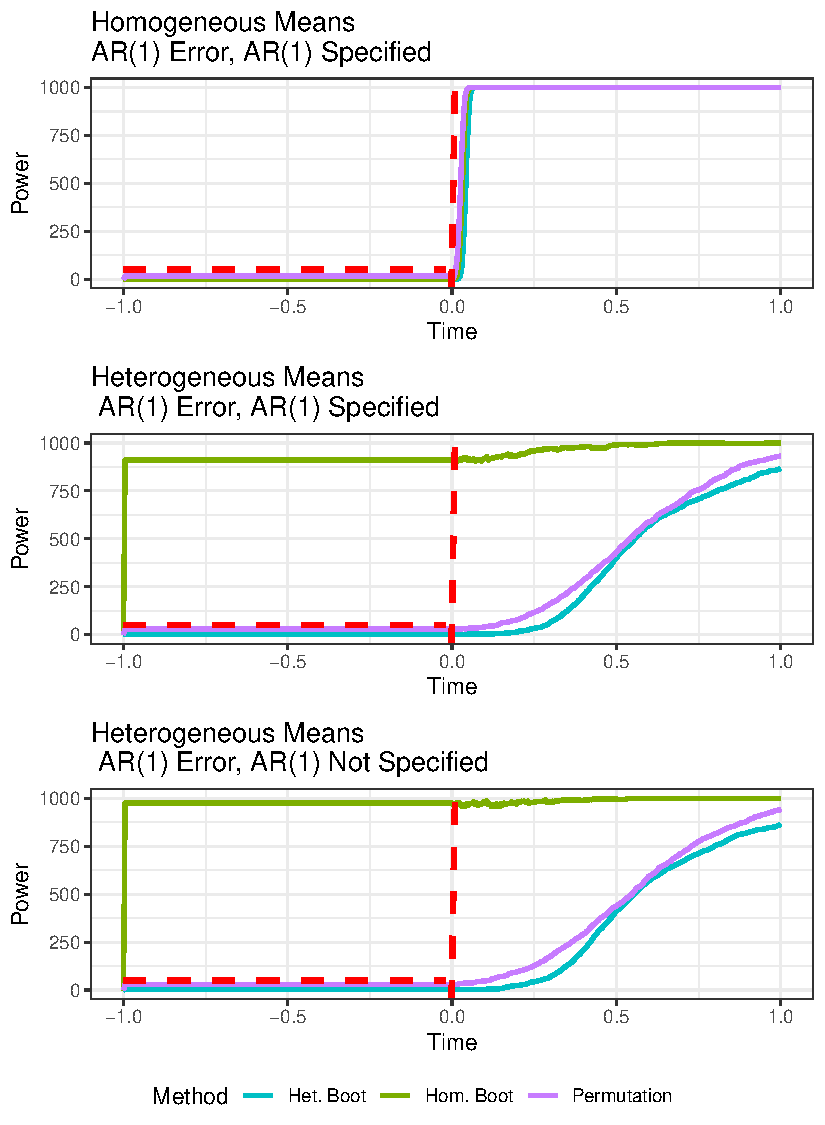
\includegraphics{typeII_time.pdf}
\caption{Observed power of each of the methods at each time in (-1,1) (not sure if better as subplots?)}
\label{fig:time_power_plot}
\end{figure}

%\begin{figure}[H]
%\centering
%    \subfigure[]{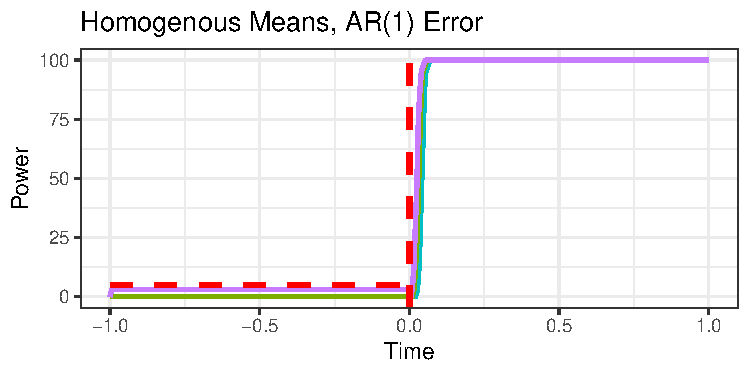
\includegraphics{type_two_error_time_a.pdf}}
%    \subfigure[]{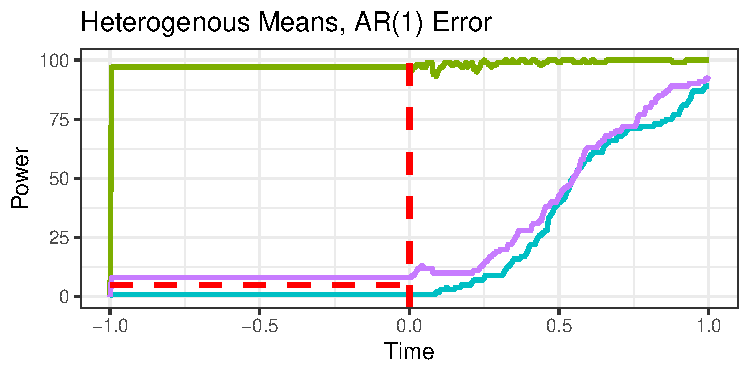
\includegraphics{type_two_error_time_b.pdf}}
%        \subfigure[]{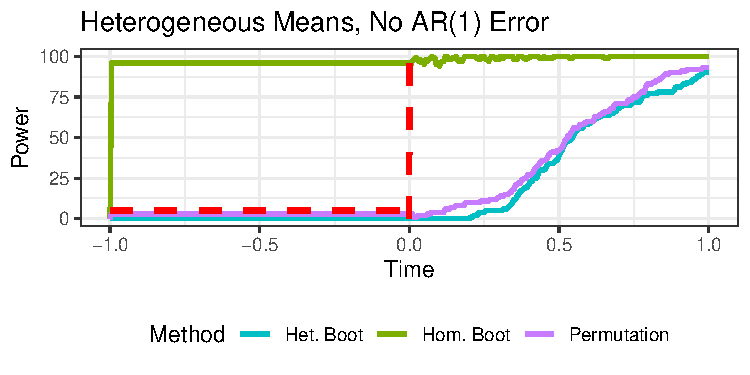
\includegraphics{type_two_error_time_c.pdf}}
%\caption{Observed power of each of the methods at each time in (-1,1)}
%\label{fig:time_power_plot}
%\end{figure}

\section{Discussion and concluding remarks}

We set out both to interrogate the validity of the homogeneous bootstrap assumptions and to propose two alternative methods that would be more robust under a greater variety of assumptions. In doing so, we demonstrated conclusively the utility of the heterogeneous bootstrap and permutation tests while also highlighting a major shortcoming of the original. It's worth noting, however, that the FWER adjustment proposed in \cite{oleson2017detecting} is still valid, if not slightly conservative, and with power similar to that of the permutation method. 

In light of the results presented, one issue of concern is addressing the fact that a version of \xt{bdots} with the homogeneous mean assumption was presented in 2018 and remained accessible on CRAN until the end of 2022. This has implications for the number of papers in which \xt{bdots} may have demonstrated significance between groups when the underlying assumptions of homogeneous mean structure did not hold, as is likely the case in all instances related to the VWP. Concurrent with this issue is the issue of identifying current users of \xt{bdots} of this change, as results found only a month ago will be profoundly different than what is seen today. At present, I am not sure the best way to address either of these. In either case, however, it will be prudent to remove this option from the \xt{bdots} package all together, as there appears to be no obvious advantage to the homogeneous bootstrap over the others in terms of either controlling the FWER or obtaining power, even when the homogeneous mean structure assumption is met.

There are several limitations of the current paper that are worthy of further investigation. First, First, limited consideration was given to the effect of sample density on the observed type I error rate or power. As the fitting function in \xt{bdots} simply returns a set of parameters, one could conceivably perform any of the methods presented on any arbitrary collection of points, whether or not any data were observed there. This extends itself to the condition in which subjects were sampled at heterogeneous time points, as may be the case in many clinical settings. What impact this may have or how to best handle these cases remains open for exploration. It is also worth investigating in greater detail what impact the re-drawing of subject specific parameters from their respective distributions has on both the FWER and power, as in several of the simulations the observed FWER was much lower than the nominal level. Particularly in the case of the permutation method which is \textit{not} seeking to estimate the group distributions, it may be worthwhile to see if a favorable trade can be made to increase the resulting power.

We conclude by noting that \xt{bdots} is now equipped with two methods to effectively control the FWER when assessing the differences in time series under a greater set of underlying assumptions, including those involving the presence of highly correlated test statistics. Further, both methods presented are robust to misspecification of the error structure while maintaining an acceptable FWER and adequate power. 

\section{Appendix -- Full Power Simulations}

Here we present the full collection of power sims, which, in addition to those given in Table~\ref{tab:power_methods} includes cases for heterogeneous means where autocorrelation is specified when fitting with \xt{bdots}. This is indicated in the ``AR(1) Specified" column. Additionally, plots giving the power at each time are presented in Figure~\ref{fig:time_power_plot_full}.

Notably from this table, we see that in the case in which the true errors are IID, there is no measurable effect on power when an autocorrelated structure is incorrectly specified.  This is similar to the opposite situation, in which the true error does have an AR(1) structure. In this case, we observe a marginal benefit to correctly specifying an AR(1) structure. This may in fact make retaining the AR(1) assumption a reasonable default in the \xt{bdots} package.

We conclude by noting that of all of the methods investigated, that using permutation testing seems to have the preferable balance between controlling the FWER and power. 


\begin{figure}
\centering
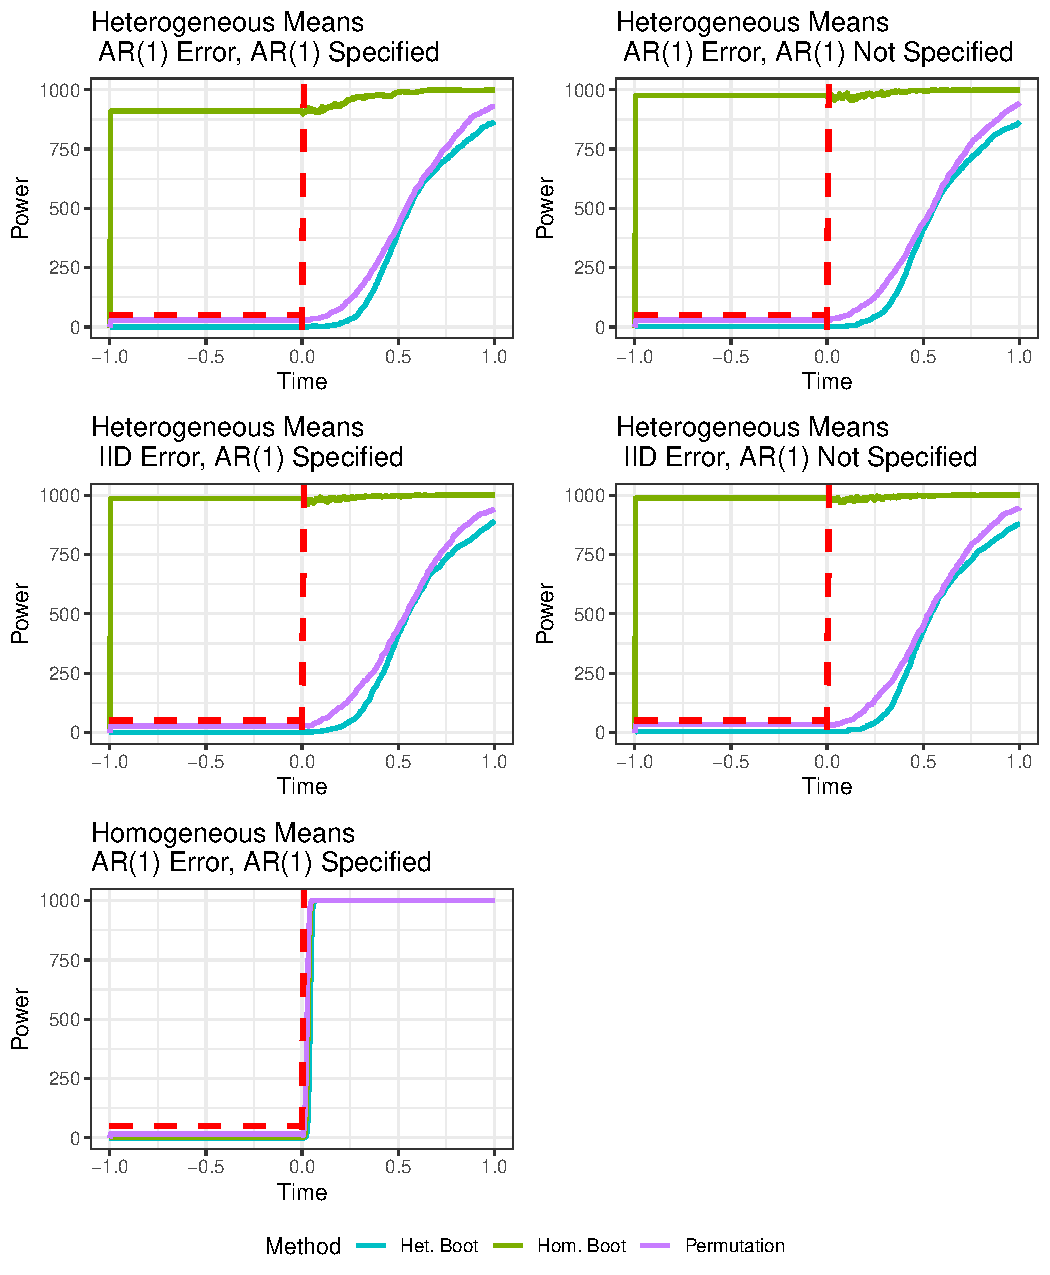
\includegraphics[scale=1]{full_power_25.pdf}
\caption{Power plots in time for each of the simulation settings. Note that in the heterogeneous means case, there is little difference when AR(1) is incorrectly specified}
\label{fig:time_power_plot_full}
\end{figure}

\begin{landscape}
\begin{table}[ht]
\centering
\begin{tabular}{llllcccccc}
  \hline
Method & Heterogeneity & AR(1) Error & AR(1) Specified & $\alpha$ & $\beta$ & 1 - $\alpha$ - $\beta$ & 1st Qu. & Median & 3rd Qu.  \\ 
  \hline
Hom. Boot & No & Yes & Yes & 0.00 & 0.00 & 1.00 & 0.025 & 0.030 & 0.035 \\ 
  Het. Boot & No & Yes & Yes & 0.00 & 0.00 & 1.00 & 0.035 & 0.040 & 0.045 \\ 
  Perm & No & Yes & Yes & 0.03 & 0.00 & 0.97 & 0.020 & 0.025 & 0.030 \\ \hline
  Hom. Boot & Yes & No & No & 0.95 & 0.00 & 0.05 & 0.005 & 0.008 & 0.010 \\ 
  Het. Boot & Yes & No & No & 0.00 & 0.01 & 0.98 & 0.260 & 0.330 & 0.480 \\ 
  Perm & Yes & No & No & 0.04 & 0.00 & 0.95 & 0.245 & 0.325 & 0.452 \\ \hline
  Hom. Boot & Yes & No & Yes & 0.98 & 0.00 & 0.02 & 0.005 & 0.008 & 0.010 \\ 
  Het. Boot & Yes & No & Yes & 0.00 & 0.01 & 0.99 & 0.261 & 0.350 & 0.475 \\ 
  Perm & Yes & No & Yes & 0.04 & 0.00 & 0.96 & 0.225 & 0.335 & 0.440 \\ \hline
  Hom. Boot & Yes & Yes & No & 0.94 & 0.00 & 0.06 & 0.005 & 0.013 & 0.015 \\ 
  Het. Boot & Yes & Yes & No & 0.01 & 0.01 & 0.98 & 0.270 & 0.370 & 0.465 \\ 
  Perm & Yes & Yes & No & 0.04 & 0.00 & 0.96 & 0.245 & 0.365 & 0.440 \\ \hline
  Hom. Boot & Yes & Yes & Yes & 0.83 & 0.00 & 0.17 & 0.021 & 0.032 & 0.040 \\ 
  Het. Boot & Yes & Yes & Yes & 0.00 & 0.01 & 0.98 & 0.250 & 0.330 & 0.450 \\ 
  Perm & Yes & Yes & Yes & 0.03 & 0.00 & 0.97 & 0.223 & 0.335 & 0.428 \\ 
   \hline
\end{tabular}
\caption{Power for methods} 
\label{tab:power_methods_full}
\end{table}
\end{landscape}

